\chapter{Universal Asynchronous Receiver-Transmitter (UART)}

\section*{Learning Objectives}
After completing this experiment, you will be able to:
\begin{itemize}[nosep]
  \item Understand the principles of asynchronous serial communication including start bits, stop bits, and data frames.
  \item Configure UART baud rate using integer and fractional divisors for precise timing.
  \item Configure GPIO pins for UART alternate function using AFSEL, PCTL, and DEN registers.
  \item Implement basic UART transmission and reception functions in C.
  \item Send and receive strings via serial communication using polling methods.
  \item Interface with a PC terminal emulator for debugging and data visualization.
  \item Calculate and verify baud rate divisors for different system clock frequencies.
  \item Understand UART FIFO buffering and status flag operations.
\end{itemize}

\section*{Experiment Overview}
This experiment introduces serial communication using the TM4C123's UART modules. You will configure UART0 for 115200 baud operation on pins PA0 (RX) and PA1 (TX), implement character and string transmission functions, and create an echo server that receives data from a PC terminal and echoes it back. By the end of this lab, you will understand how asynchronous serial communication enables data exchange between embedded systems and external devices, forming the foundation for debugging, sensor interfacing, and wireless communication modules.

\newpage
\etocsetnexttocdepth{subsubsection}
\localtableofcontents
\bigskip
\newpage

\section{Theoretical Background}

\subsection{Introduction to Serial Communication}

Serial communication is a method of transmitting data one bit at a time over a single communication line, as opposed to parallel communication which sends multiple bits simultaneously. It is widely used in embedded systems due to its simplicity, low pin count, and ability to communicate over long distances.

\subsubsection{Asynchronous vs Synchronous Communication}

Serial communication can be classified into two categories:

\begin{itemize}[nosep]
  \item \textbf{Asynchronous (UART)}: No shared clock signal; timing is established by agreed-upon baud rate. Uses start and stop bits for synchronization.
  \item \textbf{Synchronous (SPI, I\textsuperscript{2}C)}: Dedicated clock line synchronizes transmitter and receiver. More efficient but requires additional pin.
\end{itemize}

UART (Universal Asynchronous Receiver-Transmitter) is an asynchronous protocol that requires only two wires: TX (transmit) and RX (receive). It is commonly used for debugging, GPS modules, Bluetooth communication, and PC interfacing.

\subsection{UART Frame Structure}

A UART transmission consists of a \textbf{data frame} that includes:

\begin{enumerate}[nosep]
  \item \textbf{Start Bit}: Logic low (0) that signals the beginning of transmission
  \item \textbf{Data Bits}: 5 to 9 bits of actual data (typically 8 bits)
  \item \textbf{Parity Bit}: Optional error-checking bit (even, odd, or none)
  \item \textbf{Stop Bits}: Logic high (1) that signals the end of transmission (1, 1.5, or 2 bits)
\end{enumerate}

The most common configuration is \textbf{8N1}: 8 data bits, No parity, 1 stop bit.

\begin{figure}[H]
\centering
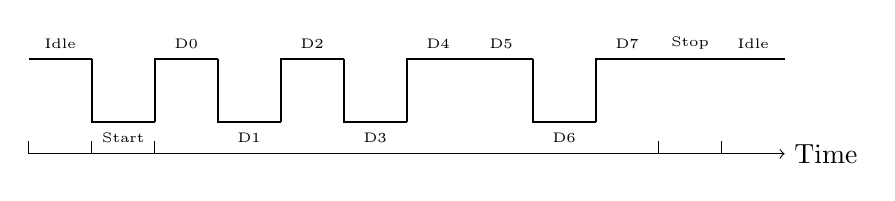
\begin{tikzpicture}[scale=0.8]
  % Idle state
  \draw[thick] (0,1) -- (1,1) node[midway,above] {\tiny Idle};
  % Start bit
  \draw[thick] (1,1) -- (1,0) -- (2,0) node[midway,below] {\tiny Start};
  % Data bits
  \draw[thick] (2,0) -- (2,1) -- (3,1) node[midway,above] {\tiny D0};
  \draw[thick] (3,1) -- (3,0) -- (4,0) node[midway,below] {\tiny D1};
  \draw[thick] (4,0) -- (4,1) -- (5,1) node[midway,above] {\tiny D2};
  \draw[thick] (5,1) -- (5,0) -- (6,0) node[midway,below] {\tiny D3};
  \draw[thick] (6,0) -- (6,1) -- (7,1) node[midway,above] {\tiny D4};
  \draw[thick] (7,1) -- (7,1) -- (8,1) node[midway,above] {\tiny D5};
  \draw[thick] (8,1) -- (8,0) -- (9,0) node[midway,below] {\tiny D6};
  \draw[thick] (9,0) -- (9,1) -- (10,1) node[midway,above] {\tiny D7};
  % Stop bit
  \draw[thick] (10,1) -- (10,1) -- (11,1) node[midway,above] {\tiny Stop};
  % Idle
  \draw[thick] (11,1) -- (12,1) node[midway,above] {\tiny Idle};
  
  % Axis
  \draw[->] (0,-0.5) -- (12,-0.5) node[right] {Time};
  \draw (0,-0.5) -- (0,-0.3);
  \draw (1,-0.5) -- (1,-0.3);
  \draw (2,-0.5) -- (2,-0.3);
  \draw (10,-0.5) -- (10,-0.3);
  \draw (11,-0.5) -- (11,-0.3);
\end{tikzpicture}
\caption{UART Frame Structure (8N1 Format)}
\label{fig:uart-frame}
\end{figure}

\subsection{Baud Rate Generation}

The \textbf{baud rate} defines the number of bits transmitted per second, measured in bits per second (bps). Common baud rates include 9600, 19200, 38400, 57600, and 115200 bps. Both transmitter and receiver must use the same baud rate for successful communication.

\subsubsection{Baud Rate Divisor Calculation}

The TM4C123 UART uses a \textbf{22-bit baud rate divisor (BRD)} consisting of a 16-bit integer part (BRDI) and a 6-bit fractional part (BRDF). This fractional divisor allows the UART to generate all standard baud rates with high precision.

The baud rate divisor is calculated from the system clock frequency as:

\begin{equation}
\text{BRD} = \text{BRDI} + \text{BRDF} = \frac{\text{UARTSysClk}}{\text{ClkDiv} \times \text{BaudRate}}
\end{equation}

where:
\begin{itemize}[nosep]
  \item \textbf{UARTSysClk}: System clock connected to UART (typically 50 MHz)
  \item \textbf{ClkDiv}: Clock divider (16 if HSE = 0 in UARTCTL, or 8 if HSE = 1)
  \item \textbf{BaudRate}: Desired baud rate (e.g., 115200 bps)
\end{itemize}

The integer part (BRDI) is loaded into the \texttt{UARTIBRD} register, and the fractional part is calculated and loaded into the \texttt{UARTFBRD} register using:

\begin{equation}
\text{UARTFBRD[DIVFRAC]} = \text{integer}(\text{BRDF} \times 64 + 0.5)
\end{equation}

The multiplication by 64 and addition of 0.5 accounts for the 6-bit fractional representation and rounding errors.

\subsubsection{Baud Rate Generation Process}

The UART generates an internal baud rate reference clock at either 8x or 16x the target baud rate (called Baud8 or Baud16), depending on the HSE bit setting. This reference clock is then divided by 8 or 16 to generate the actual transmit clock and is used for error detection during receive operations.



\subsubsection{Calculation Example}

\textbf{Example}: For 115200 baud with 50 MHz system clock and ClkDiv = 16 (default, HSE = 0):

\begin{align*}
\text{BRD} &= \frac{50{,}000{,}000}{16 \times 115{,}200} = \frac{50{,}000{,}000}{1{,}843{,}200} = 27.1267361 \\
\text{BRDI} &= 27 \\
\text{BRDF} &= 0.1267361 \\
\text{UARTFBRD[DIVFRAC]} &= \text{integer}(0.1267361 \times 64 + 0.5) \\
&= \text{integer}(8.111 + 0.5) = \text{integer}(8.611) = 8
\end{align*}

Therefore: \texttt{UARTIBRD = 27} and \texttt{UARTFBRD = 8}

The actual baud rate achieved can be verified:
\begin{equation}
\text{Actual Baud Rate} = \frac{50{,}000{,}000}{16 \times (27 + 8/64)} = \frac{50{,}000{,}000}{16 \times 27.125} = 115{,}207.4 \text{ bps}
\end{equation}

This gives an error of only 0.0064\%, well within acceptable tolerance for reliable communication.

\subsection{TM4C123 UART Modules}

The TM4C123GH6PM provides \textbf{eight UART modules} (UART0-UART7) with the following features:

\begin{itemize}[nosep]
  \item \textbf{Programmable Baud Rate}: Generated from system clock with 16-bit divisor
  \item \textbf{Data Format}: 5 to 9 data bits, optional parity (even, odd, stick), 1 or 2 stop bits
  \item \textbf{FIFO Buffers}: 16-byte transmit and receive FIFOs for reduced interrupt overhead
  \item \textbf{Full-Duplex Operation}: Simultaneous transmission and reception
  \item \textbf{Error Detection}: Framing, parity, overrun, and break detection
  \item \textbf{Interrupt Generation}: Configurable interrupts for TX, RX, and error conditions
  \item \textbf{DMA Support}: $\mu$DMA channels for high-speed data transfer
  \item \textbf{IrDA and ISO 7816}: Optional infrared and smart card support
  \item \textbf{9-Bit Mode}: For RS-485 multi-drop networks
\end{itemize}

\subsubsection{FIFO Operation}

Each UART module contains two 16x8 FIFOs: one for transmit and one for receive. Both FIFOs are accessed through the \texttt{UARTDR} register. Read operations return a 12-bit value consisting of 8 data bits and 4 error flags, while write operations place 8-bit data into the transmit FIFO.


\textbf{FIFO Status Monitoring}:

FIFO status can be monitored using two registers:

\begin{enumerate}[nosep]
  \item \textbf{UARTFR (Flag Register)}: Contains empty and full flags
  \begin{itemize}[nosep]
    \item \textbf{TXFE} (bit 7): Transmit FIFO Empty
    \item \textbf{TXFF} (bit 5): Transmit FIFO Full
    \item \textbf{RXFE} (bit 4): Receive FIFO Empty
    \item \textbf{RXFF} (bit 6): Receive FIFO Full
  \end{itemize}
  
\end{enumerate}



\subsubsection{UART Pin Mapping}

Each UART module is connected to specific GPIO pins. The table below shows the default pin assignments:

\begin{table}[H]
\centering
\small
\begin{tabular}{ccc}
\toprule
\textbf{UART Module} & \textbf{TX Pin} & \textbf{RX Pin} \\
\midrule
UART0 & PA1 & PA0 \\
UART1 & PB1 & PB0 \\
UART2 & PD7 & PD6 \\
UART3 & PC7 & PC6 \\
UART4 & PC5 & PC4 \\
UART5 & PE5 & PE4 \\
UART6 & PD5 & PD4 \\
UART7 & PE1 & PE0 \\
\bottomrule
\end{tabular}
\caption{UART Pin Assignments}
\end{table}

\textbf{Note}: UART0 on PA0/PA1 is commonly used because it connects to the LaunchPad's on-board USB-to-Serial converter, allowing direct PC communication via USB cable.


\subsection{UART Registers}

The TM4C123 UART modules are configured through memory-mapped registers. Key registers include:

\bigskip
\subsubsection*{RCGCUART — UART Run Mode Clock Gating Control}
Enables clock for UART modules. Each bit corresponds to a UART module (1 = enable, 0 = disable).

\begin{figure}[H]
\centering
\begin{bytefield}[endianness=big,bitwidth=\widthof{\tiny{~UART0~}}]{16}
\bitheader[lsb=16]{16-31} \\
\bitbox{16}[bgcolor=gray!10]{\tiny{reserved}} \\
\bitheader{0-15} \\
\bitbox{8}[bgcolor=gray!10]{\tiny{reserved}} & 
\bitbox{1}{\tiny{R7}} & \bitbox{1}{\tiny{R6}} & \bitbox{1}{\tiny{R5}} & \bitbox{1}{\tiny{R4}} & 
\bitbox{1}{\tiny{R3}} & \bitbox{1}{\tiny{R2}} & \bitbox{1}{\tiny{R1}} & \bitbox{1}{\tiny{R0}} \\
\end{bytefield}
\caption{RCGCUART Register — UART Run Mode Clock Gating Control}
\end{figure}

\bigskip
\subsubsection*{UARTCTL — UART Control}
Configures UART operation including enable, transmit enable, and receive enable.

\begin{figure}[H]
\centering
\begin{bytefield}[endianness=big,bitwidth=\widthof{\tiny{~UART0~}}]{16}
\bitheader[lsb=16]{16-31} \\
\bitbox{16}[bgcolor=gray!10]{\tiny{reserved}} \\
\bitheader{0-15} \\
\bitbox{1}{\tiny{CTSEN}} & \bitbox{1}{\tiny{RTSEN}} & \bitbox{2}[bgcolor=gray!10]{\tiny{reserved}} & 
\bitbox{1}{\tiny{RTS}} & \bitbox{1}[bgcolor=gray!10]{\tiny{reserved}} & 
\bitbox{1}{\tiny{RXE}} & \bitbox{1}{\tiny{TXE}} & \bitbox{1}{\tiny{LBE}} & 
\bitbox{1}[bgcolor=gray!10]{\tiny{reserved}} & \bitbox{1}{\tiny{HSE}}& \bitbox{1}{\tiny{EOT}}& \bitbox{1}{\tiny{SMART}}& \bitbox{1}{\tiny{SIRLP}}& \bitbox{1}{\tiny{SIREN}}& \bitbox{1}{\miniscule{UARTEN}} \\
\end{bytefield}
\caption{UARTCTL Register — UART Control}
\end{figure}

Where:
\begin{itemize}[nosep]
  \item \textbf{UARTEN} (bit 0): UART Enable (1 = enable, 0 = disable)
  \item \textbf{TXE} (bit 8): Transmit Enable (1 = enable transmitter)
  \item \textbf{RXE} (bit 9): Receive Enable (1 = enable receiver)
  \item \textbf{HSE} (bit 5): High-Speed Enable (1 = baud rate clock = SysClk/8, 0 = SysClk/16)
\end{itemize}
\bigskip
\subsubsection*{UARTIBRD — UART Integer Baud-Rate Divisor}
Contains the integer part of the baud rate divisor.

\begin{figure}[H]
\centering
\begin{bytefield}[endianness=big,bitwidth=\widthof{\tiny{~UART0~}}]{16}
\bitheader[lsb=16]{16-31} \\
\bitbox{16}[bgcolor=gray!10]{\tiny{reserved}} \\
\bitheader{0-15} \\
\bitbox{16}{\tiny{DIVINT}} \\
\end{bytefield}
\caption{UARTIBRD Register — UART Integer Baud-Rate Divisor}
\end{figure}

Where:
\begin{itemize}[nosep]
  \item \textbf{DIVINT}: Integer baud rate divisor (0-65535)
\end{itemize}

\bigskip
\subsubsection*{UARTFBRD — UART Fractional Baud-Rate Divisor}
Contains the fractional part of the baud rate divisor.

\begin{figure}[H]
\centering
\begin{bytefield}[endianness=big,bitwidth=\widthof{\tiny{~UART0~}}]{16}
\bitheader[lsb=16]{16-31} \\
\bitbox{16}[bgcolor=gray!10]{\tiny{reserved}} \\
\bitheader{0-15} \\
\bitbox{10}[bgcolor=gray!10]{\tiny{reserved}} & \bitbox{6}{\tiny{DIVFRAC}} \\
\end{bytefield}
\caption{UARTFBRD Register — UART Fractional Baud-Rate Divisor}
\end{figure}

Where:
\begin{itemize}[nosep]
  \item \textbf{DIVFRAC}: Fractional baud rate divisor (0-63)
\end{itemize}

\bigskip
\subsubsection*{UARTLCRH — UART Line Control}
Configures data format including word length, FIFO enable, parity, and stop bits.

\begin{figure}[H]
\centering
\begin{bytefield}[endianness=big,bitwidth=\widthof{\tiny{~UART0~}}]{16}
\bitheader[lsb=16]{16-31} \\
\bitbox{16}[bgcolor=gray!10]{\tiny{reserved}} \\
\bitheader{0-15} \\
\bitbox{8}[bgcolor=gray!10]{\tiny{reserved}} & \bitbox{1}{\tiny{SPS}} & \bitbox{2}{\tiny{WLEN}} & 
\bitbox{1}{\tiny{FEN}} & \bitbox{1}{\tiny{STP2}} & \bitbox{1}{\tiny{EPS}} & 
\bitbox{1}{\tiny{PEN}} & \bitbox{1}{\tiny{BRK}} \\
\end{bytefield}
\caption{UARTLCRH Register — UART Line Control}
\end{figure}

Where:
\begin{itemize}[nosep]
  \item \textbf{WLEN} (bits 6-5): Word Length (0x3 = 8 bits, 0x2 = 7 bits, 0x1 = 6 bits, 0x0 = 5 bits)
  \item \textbf{FEN} (bit 4): FIFO Enable (1 = enable 16-byte FIFOs, 0 = disable)
  \item \textbf{STP2} (bit 3): Two Stop Bits (1 = two stop bits, 0 = one stop bit)
  \item \textbf{EPS} (bit 2): Even Parity Select (1 = even parity, 0 = odd parity)
  \item \textbf{PEN} (bit 1): Parity Enable (1 = enable parity, 0 = no parity)
  \item \textbf{BRK} (bit 0): Send Break (1 = send break condition)
\end{itemize}

\textbf{Common Configuration (8N1 with FIFO)}:
\begin{itemize}[nosep]
  \item WLEN = 0x3 (8 bits)
  \item FEN = 1 (FIFO enabled)
  \item STP2 = 0 (one stop bit)
  \item PEN = 0 (no parity)
\end{itemize}
Result: \texttt{UARTLCRH = 0x60} (0b01100000)

\bigskip
\subsubsection*{UARTCC — UART Clock Configuration}
Selects the clock source for UART baud rate generation.

\begin{figure}[H]
\centering
\begin{bytefield}[endianness=big,bitwidth=\widthof{\tiny{~UART0~}}]{16}
\bitheader[lsb=16]{16-31} \\
\bitbox{16}[bgcolor=gray!10]{\tiny{reserved}} \\
\bitheader{0-15} \\
\bitbox{12}[bgcolor=gray!10]{\tiny{reserved}} & \bitbox{4}{\tiny{CS}} \\
\end{bytefield}
\caption{UARTCC Register — UART Clock Configuration}
\end{figure}

Where:
\begin{itemize}[nosep]
  \item \textbf{CS} (bits 3-0): Clock Source
  \begin{itemize}[nosep]
    \item 0x0 = System clock (default, recommended)
    \item 0x5 = PIOSC (16 MHz internal oscillator)
  \end{itemize}
\end{itemize}

\bigskip
\subsubsection*{UARTFR — UART Flag Register}
Contains status flags for transmit/receive operations.

\begin{figure}[H]
\centering
\begin{bytefield}[endianness=big,bitwidth=\widthof{\tiny{~UART0~}}]{16}
\bitheader[lsb=16]{16-31} \\
\bitbox{16}[bgcolor=gray!10]{\tiny{reserved}} \\
\bitheader{0-15} \\
\bitbox{8}[bgcolor=gray!10]{\tiny{reserved}} & \bitbox{1}{\tiny{TXFE}} & \bitbox{1}{\tiny{RXFF}} & 
\bitbox{1}{\tiny{TXFF}} & \bitbox{1}{\tiny{RXFE}} & \bitbox{1}{\tiny{BUSY}} & 
\bitbox{2}[bgcolor=gray!10]{\tiny{reserved}} & \bitbox{1}{\tiny{CTS}}\\
\end{bytefield} 
\caption{UARTFR Register — UART Flag Register}
\end{figure}

Where:
\begin{itemize}[nosep]
  \item \textbf{TXFE} (bit 7): Transmit FIFO Empty (1 = empty, 0 = not empty)
  \item \textbf{RXFF} (bit 6): Receive FIFO Full (1 = full, 0 = not full)
  \item \textbf{TXFF} (bit 5): Transmit FIFO Full (1 = full, 0 = not full)
  \item \textbf{RXFE} (bit 4): Receive FIFO Empty (1 = empty, 0 = not empty)
  \item \textbf{BUSY} (bit 3): UART Busy (1 = transmitting, 0 = idle)
\end{itemize}

\textbf{Usage}:
\begin{itemize}[nosep]
  \item Before transmitting: Wait while \texttt{TXFF = 1} (transmit FIFO full)
  \item Before receiving: Wait while \texttt{RXFE = 1} (receive FIFO empty)
\end{itemize}

\bigskip
\subsubsection*{UARTDR — UART Data Register}
Contains the data to transmit or received data. Reading removes data from RX FIFO; writing adds to TX FIFO.

\begin{figure}[H]
\centering
\begin{bytefield}[endianness=big,bitwidth=\widthof{\tiny{~UART0~}}]{16}
\bitheader[lsb=16]{16-31} \\
\bitbox{16}[bgcolor=gray!10]{\tiny{reserved}} \\
\bitheader{0-15} \\
 \bitbox{4}[bgcolor=gray!10]{\tiny{reserved}} 
 &\bitbox{1}{\tiny{OE}} & \bitbox{1}{\tiny{BE}} & \bitbox{1}{\tiny{PE}} & \bitbox{1}{\tiny{FE}}
 & \bitbox{8}{\tiny{DATA}} \\
\end{bytefield}
\caption{UARTDR Register — UART Data Register}
\end{figure}

Where:
Data is contained in the lower 8 bits. The upper 4 bits indicate error flags:
\begin{itemize}[nosep]
  \item \textbf{FE} (bit 3): Framing Error
  \item \textbf{PE} (bit 2): Parity Error
  \item \textbf{BE} (bit 1): Break Error
  \item \textbf{OE} (bit 0): Overrun Error
  \item \textbf{DATA} (bits 7-0): Received or Transmit Data
\end{itemize}
\newpage
\section{Procedure}

\subsection{Configuration Steps}

Configuring UART0 on the TM4C123 microcontroller involves two stages:

\subsubsection{GPIO Pin Configuration}

To prepare GPIO pins for UART function:

\begin{enumerate}[nosep]
\item Enable the clock for UART0 module and GPIO Port A by setting the appropriate bits in the \texttt{RCGCUART} and \texttt{RCGCGPIO} registers.
\item Enable alternate function on PA0 (RX) and PA1 (TX) using the \texttt{GPIOAFSEL} register.
\item Configure the UART function encoding in the \texttt{GPIOPCTL} register (encoding = 1 for UART).
\item Enable digital function for PA0 and PA1 pins by setting bits in the \texttt{GPIODEN} register.
\end{enumerate}

\subsubsection{UART Module Setup}

After the pins are configured, the UART module must be initialized:

\begin{enumerate}[nosep]
\item Disable the UART by clearing all bits in the \texttt{UARTCTL} register to prevent undefined behavior during configuration.
\item Calculate the baud rate divisor values. For 115200 baud at 50 MHz: BRD = 50,000,000 / (16 x 115,200) = 27.1267361, giving IBRD = 27 and FBRD = 8.
\item Write the integer baud rate divisor to the \texttt{UARTIBRD} register.
\item Write the fractional baud rate divisor to the \texttt{UARTFBRD} register.
\item Configure the line control register (\texttt{UARTLCRH}) for 8 data bits, no parity, one stop bit, and FIFO enable (value = 0x60). Writing to this register latches the baud rate configuration.
\item Select the clock source by writing to the \texttt{UARTCC} register (0 = system clock).
\item Enable the UART, transmitter, and receiver by setting UARTEN, TXE, and RXE bits in the \texttt{UARTCTL} register.
\end{enumerate}

\newpage
\subsection{UART0 Initialization and Code Implementation}

The provided code includes three files demonstrating complete UART functionality:

\begin{itemize}[nosep]
  \item \texttt{uart.h}: Function prototypes and pin definitions
  \item \texttt{uart.c}: Implementation of UART initialization, read, and write functions
  \item \texttt{main.c}: Echo server application
\end{itemize}
\pagestyle{empty} % hide page numbers (and headers/footers if any)
\smallskip
\paragraph{UART Header File (\texttt{uart.h})} \hfill

\lstinputlisting[language=C, caption=UART Header File]{snippets/uart/uart.h}
\smallskip
\paragraph{UART Implementation File (\texttt{uart.c})} \hfill

\lstinputlisting[language=C, caption=UART Implementation]{snippets/uart/uart.c}
\smallskip
\paragraph{Echo Server Main Program (\texttt{main.c})} \hfill

\lstinputlisting[language=C, caption=Echo Server Main Program]{snippets/uart/main.c}
\pagestyle{plain} % hide page numbers (and headers/footers if any)

